Global ocean models are integrated over decadal time scales, which constrains the horizontal and temporal resolution that can be used in global simulations. As a result, many dynamically important processes are only partly resolved or remain unresolved, including mesoscale eddies with scales of approximately 10--100 km, mixed-layer instabilities, and submesoscale fronts. These processes influence heat transport, circulation, restratification, and tracer exchange \citep{boccaletti2007mixed,foxkemper2008mle,thomas2008submesoscale,taylor2023submesoscale}. Their effects must therefore be represented through parameterizations whose behavior strongly depends on model resolutions \citep{hallberg2013using}, the consequences of which are particularly apparent near coastal fronts, river plumes, shelf breaks, and western boundary currents, where circulation and tracer pathways can remain sensitive to grid spacing \citep{chassignet2017impact}.

One-way global-to-regional coupling provides a means of increasing resolution over a selected regional domain without applying that restrictive resolution specification throughout the global ocean. Here, the ocean component of the Energy Exascale Earth System Model (E3SM)~\citep{golaz2019e3sm}, \MPAS ocean \citep{ringler2013multi,hoch2020MPAS}, supplies the evolving large-scale state, including the regional initial condition and lateral boundary fields. The Regional Ocean Modeling System (\ROMS)~\citep{shchepetkin2005regional} is then integrated on a finer regional grid, and coupled to the global ocean system to receive consistent conditions. The regional domain can include bathymetry and coastline geometry that are not fully resolved by the \MPAS mesh, thereby improving the representation of local circulation and nearshore structure. Grid refinement alone, however, does not add the information absent from the global solutions. For example, conservative downscaling alone cannot recover unresolved fronts, stratification, and boundary variability, and this is a result of the regional model evolution of state with the right forcing conditions.
%develops must be interpreted separately from the information that the  \MPAS actually supplied: refining the regional grid cannot reconstruct fronts, stratification, or boundary variability absent from the  \MPAS state.


Regional nesting and downscaling methods have been developed previously for coupled global model settings. \citet{penven2006embedding} described a one-way \ROMS embedding procedure in which initial and lateral boundary conditions were derived from a coarser parent solution, while \citet{mason2010nesting} extended offline nesting methods to regional grids. Later work considered online and two-way approaches, including feedback from the regional model to the parent domain \citep{debreu2008embedding,debreu2012nesting}. These methods established practical approaches for ocean nesting, but the present problem differs in several respects. \MPAS ocean model uses a variable-resolution unstructured horizontal mesh, whereas \ROMS uses a structured, curvilinear grid and terrain-following vertical coordinates. Coupling the models therefore requires transfers that are consistent not only in the horizontal plane, but also across the three-dimensional water-column geometries during the entire coupled transient simulation. \TODOc{Need to add more details on how this work differs from the previous ones}


%SCRIP introduced first- and second-order conservative remapping on spherical grids~\citep{jones1999scrip}, while the TempestRemap linear-map framework generalized consistency and conservation to arbitrary meshes and orders~\citep{ullrich2015arbitrary,ullrich2016tempestremap}. High-order regridding between generalized ocean vertical coordinates addressed the axial part of the problem~\citep{white2009highorder}; applying horizontal and vertical transfer together still requires a consistent representation of the two three-dimensional column geometries.

General coupling frameworks such as ESMF provide component interfaces, field definitions, grid descriptions, and regridding services for Earth-system applications \citep{hill2004esmf}. MCT provides parallel data structures and communication patterns for coupled models \citep{larson2005mct}, and its use in COAWST supports coupled regional ocean--atmosphere--wave--sediment simulations \citep{warner2010coawst}. We instead build on the new E3SM coupler based on the Mesh Oriented datABase (\MOAB)~\citep{moab521_2020}, which provides a complete topological representation of the mesh and interfaces to define and query coupled fields as tags on mesh entities directly. We build on \MOAB's scalable, conservative and high-order remapping capabilities~\citep{mahadevan2020coupling} to implement verifiable \MPAS{}-to-\ROMS{} transfers for one-way multiscale simulation. The volumetric remapping algorithm we design uses a tensor-product formulation, separating the horizontal and vertical parts of the mesh topology and field description. This separation is what makes the three-dimensional transfer affordable: it replaces a full three-dimensional cell intersection with a reused horizontal map and an independent column operator, while still accommodating the variable resolution of the unstructured \MPAS mesh.

We develop and evaluate an offline, one-way workflow that applies a normalized horizontal map followed by a conservative vertical remap. Because the transfer is expressed as sparse operators applied to tagged mesh entities, the same construction can be driven in an online, in-memory configuration without changing the verification presented here, which concerns the accuracy of the transferred fields rather than the mechanism by which they are exchanged. We present a set of regional refinement experiments that identify when a finer \ROMS mesh improves the transferred state and when the fixed \MPAS representation becomes the limiting factor, which is what determines where refinement is worth its cost when nesting regional models within global ocean models.


\begin{figure}[htbp]
	\centering
	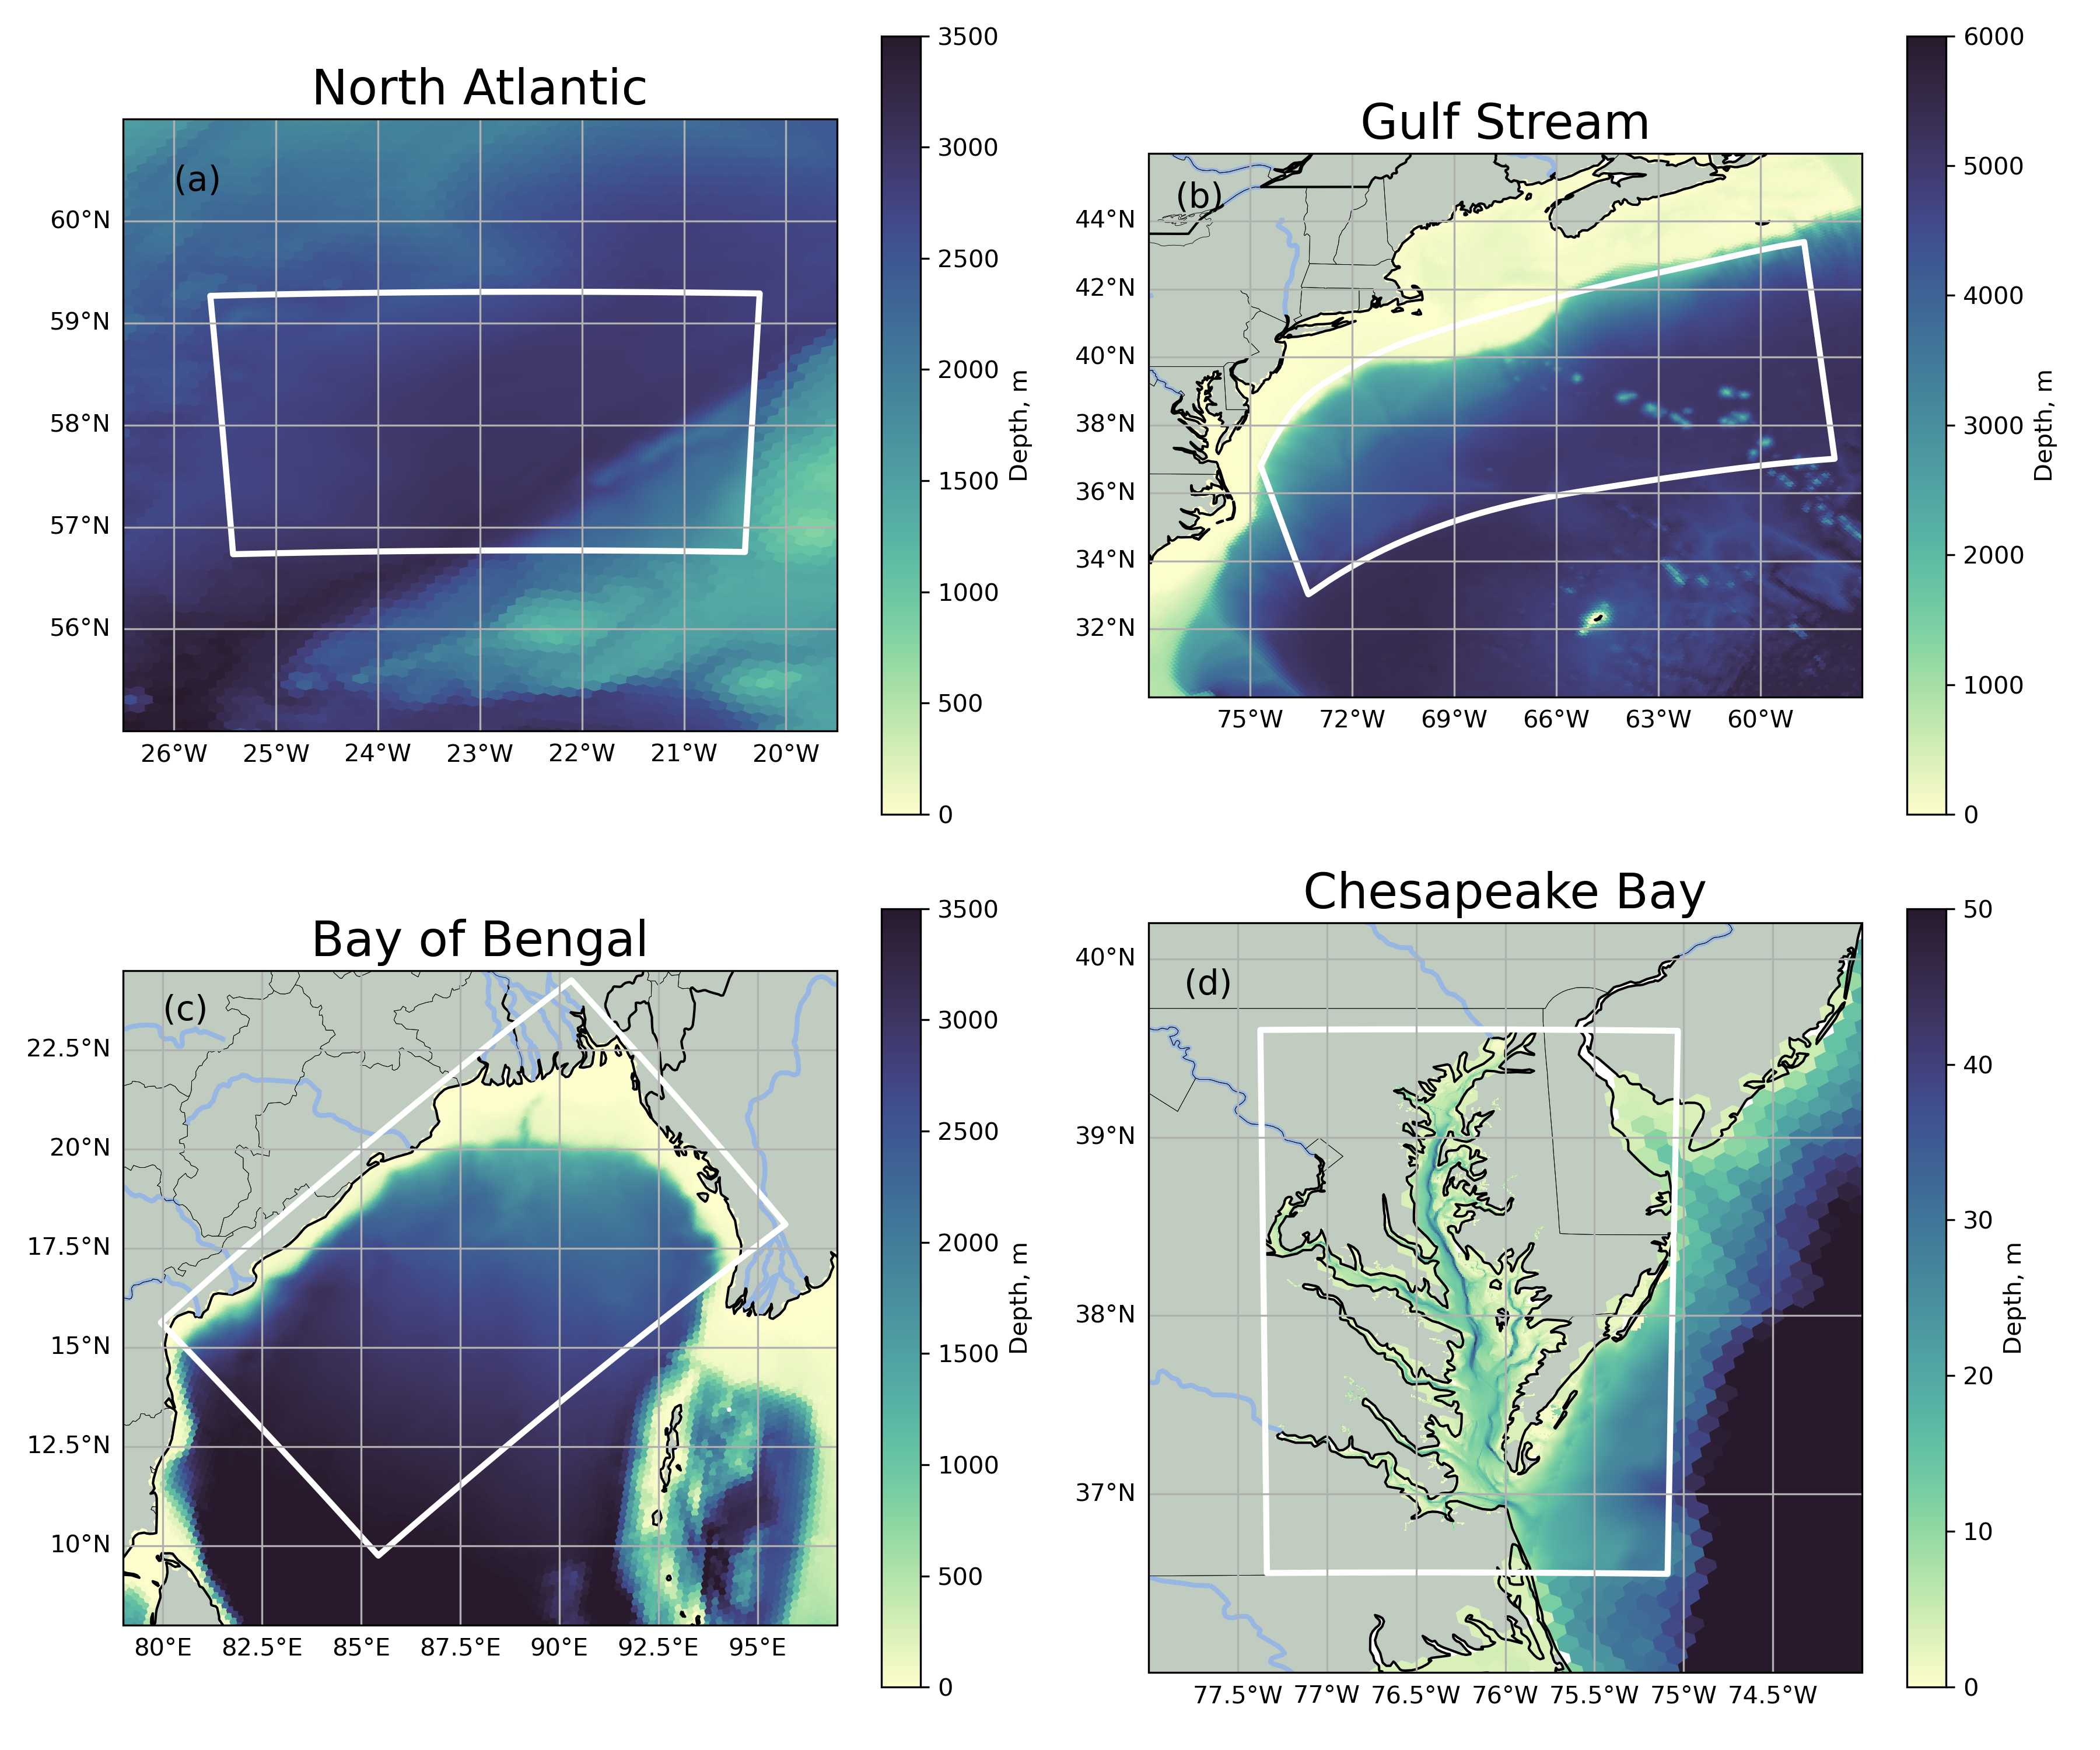
\includegraphics[width=\textwidth]{Figures/model_bathymetries_v20260629.png}
	\caption{Combined \MPAS and \ROMS bathymetries for the four application domains.}
	\label{fig:zed_comparison}
\end{figure}


The experiments reported here use four \ROMS regional domains, ordered so that each introduces a further complication for the transfer: land masks, steep bathymetric gradients, and \ROMS cells progressively smaller than anything the \MPAS mesh resolves. Their characteristic lengths range from \SI{4}{\kilo\metre} to sub-kilometre (\SI{0.6}{\kilo\metre}) estuarine scales.

The first is a North Atlantic implementation of the Near Inertial Shear and Kinetic Energy in the North Atlantic Experiment (NISKINe) model \citep{simmons2024niskine}, designed to study the generation, propagation, and dissipation of near-inertial waves and their interaction with mesoscale and submesoscale structure in the Iceland Basin. Its characteristic length is \SI{2}{\kilo\metre} over water approximately \SI{2750}{\metre} deep and carries no land mask, so it exercises the transfer with neither masking nor sharp topography.

The Gulf Stream domain adds bathymetric relief. Its curvilinear mesh, with a characteristic length of \SI{1.6}{\kilo\metre}, follows the meandering path of the western boundary current, and it also carries no land mask, but including the southern edge of Georges Bank gives it substantially sharper bathymetric gradients than the open-ocean case.
%
The third domain covers most of the Bay of Bengal with a characteristic length of \SI{4}{\kilo\metre} and adds a nearshore setting: land masks on all sides, steep bathymetric gradients, and river inputs drawn from the GloFAS-ERA5 global river discharge reanalysis \citep{harrigan2020glofas}. The fourth is the Chesapeake Bay application developed to study the sensitivity of estuarine hypoxia to external physical forcing \citep{st2024sensitivity}. Its estuarine scales fall well below what the local \MPAS grid represents and much of the domain is masked in \MPAS, so it places the greatest demand on the transfer of the four. Their geographic extent and bathymetric characteristics are shown in Fig.~\ref{fig:zed_comparison}.


\TODOc{Kyle/Rob: Add more background/motivation on \ROMS and how having this downscaling ability can help better understand ocean dynamcis in regions of interest}
